% Method Overview: Dynamic Difficulty-Aware Curriculum Learning with Boundary Refinement
% Compile with: pdflatex fig_architecture.tex
\documentclass[border=5pt]{standalone}
\usepackage{tikz}
\usepackage{amsmath,amssymb}
\usetikzlibrary{arrows.meta, positioning, fit, backgrounds, calc, shapes.geometric,
                 decorations.pathreplacing, patterns}

\definecolor{encblue}{HTML}{4A90D9}
\definecolor{decgreen}{HTML}{27AE60}
\definecolor{headred}{HTML}{E74C3C}
\definecolor{headorange}{HTML}{E67E22}
\definecolor{lossyellow}{HTML}{F1C40F}
\definecolor{diffpurple}{HTML}{8E44AD}
\definecolor{sampgray}{HTML}{7F8C8D}
\definecolor{currteal}{HTML}{16A085}
\definecolor{inputbg}{HTML}{ECF0F1}
\definecolor{lightblue}{HTML}{D6EAF8}
\definecolor{lightgreen}{HTML}{D5F5E3}
\definecolor{lightred}{HTML}{FADBD8}
\definecolor{lightyellow}{HTML}{FEF9E7}
\definecolor{lightpurple}{HTML}{E8DAEF}

\begin{document}
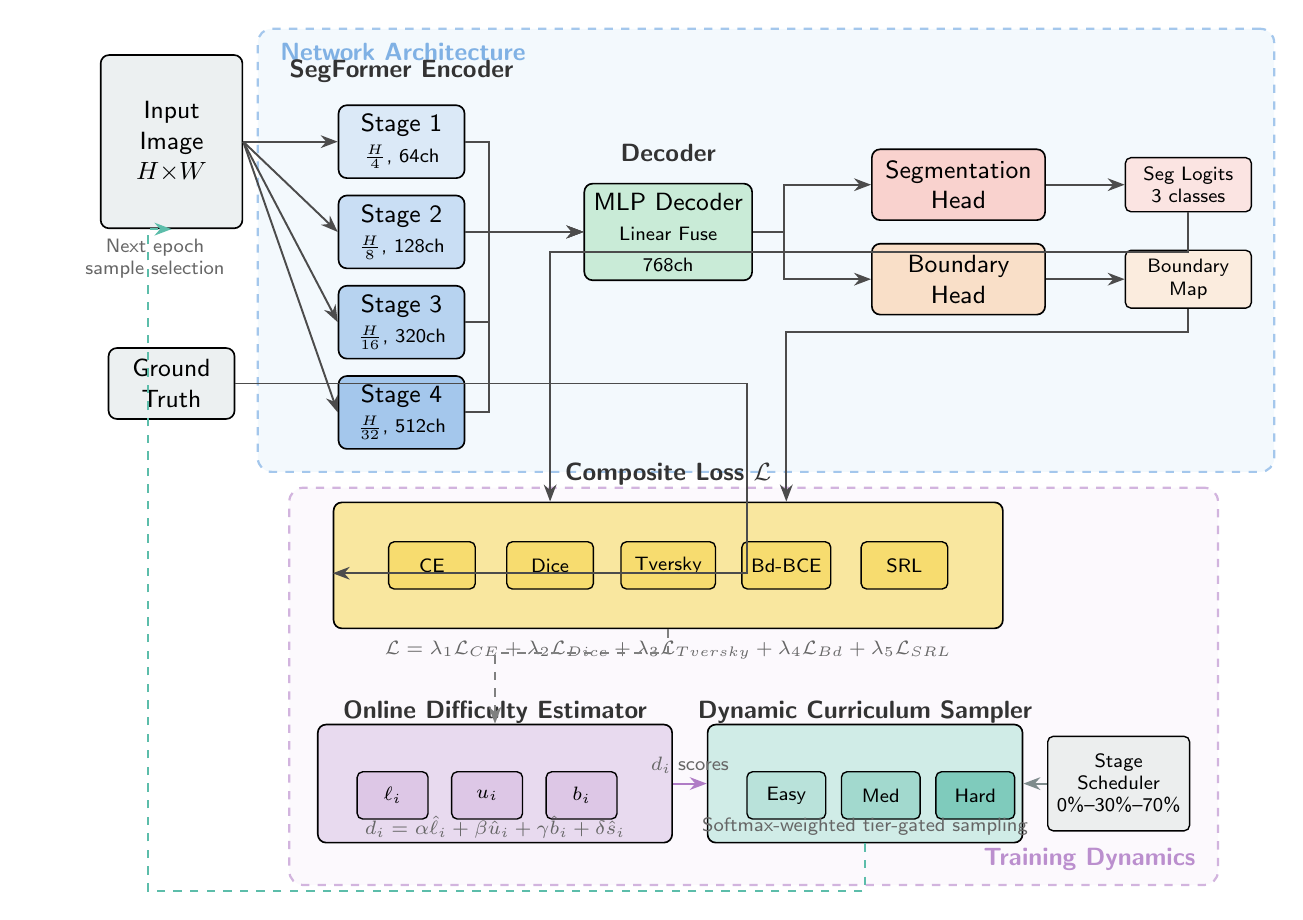
\begin{tikzpicture}[
    >=Stealth,
    node distance=0.8cm,
    block/.style={draw, rounded corners=3pt, minimum height=0.9cm,
                  minimum width=2.2cm, align=center, font=\small\sffamily,
                  line width=0.6pt},
    smallblock/.style={draw, rounded corners=2pt, minimum height=0.6cm,
                       minimum width=1.6cm, align=center, font=\scriptsize\sffamily,
                       line width=0.5pt},
    arrow/.style={->, line width=0.7pt, color=black!70},
    dasharrow/.style={->, line width=0.7pt, dashed, color=black!50},
    label/.style={font=\scriptsize\sffamily, color=black!60},
    grouplabel/.style={font=\small\sffamily\bfseries, color=black!80},
]

% ============================================================
% INPUT
% ============================================================
\node[block, fill=inputbg, minimum width=1.8cm, minimum height=2.2cm] (input) {Input\\Image\\$H{\times}W$};

% ============================================================
% ENCODER (SegFormer)
% ============================================================
\node[block, fill=encblue!20, right=1.2cm of input, minimum width=1.6cm, minimum height=0.5cm] (enc1) {Stage 1\\{\scriptsize$\frac{H}{4}$, 64ch}};
\node[block, fill=encblue!30, below=0.2cm of enc1, minimum width=1.6cm, minimum height=0.5cm] (enc2) {Stage 2\\{\scriptsize$\frac{H}{8}$, 128ch}};
\node[block, fill=encblue!40, below=0.2cm of enc2, minimum width=1.6cm, minimum height=0.5cm] (enc3) {Stage 3\\{\scriptsize$\frac{H}{16}$, 320ch}};
\node[block, fill=encblue!50, below=0.2cm of enc3, minimum width=1.6cm, minimum height=0.5cm] (enc4) {Stage 4\\{\scriptsize$\frac{H}{32}$, 512ch}};

% Encoder group label
\node[grouplabel, above=0.15cm of enc1] (enc_label) {SegFormer Encoder};

% Input arrows
\draw[arrow] (input.east) -- (enc1.west);
\draw[arrow] (input.east) -- (enc2.west);
\draw[arrow] (input.east) -- (enc3.west);
\draw[arrow] (input.east) -- (enc4.west);

% ============================================================
% DECODER
% ============================================================
\node[block, fill=decgreen!25, right=1.5cm of enc2, minimum width=2.0cm, minimum height=1.0cm]
    (decoder) {MLP Decoder\\{\scriptsize Linear Fuse}\\{\scriptsize 768ch}};

\node[grouplabel, above=0.15cm of decoder] {Decoder};

% Encoder to decoder
\draw[arrow] (enc1.east) -- ++(0.3,0) |- (decoder.west);
\draw[arrow] (enc2.east) -- (decoder.west);
\draw[arrow] (enc3.east) -- ++(0.3,0) |- (decoder.west);
\draw[arrow] (enc4.east) -- ++(0.3,0) |- (decoder.west);

% ============================================================
% HEADS (Segmentation + Boundary)
% ============================================================
\node[block, fill=headred!25, right=1.5cm of decoder, yshift=0.6cm,
      minimum width=2.2cm] (seghead) {Segmentation\\Head};
\node[block, fill=headorange!25, right=1.5cm of decoder, yshift=-0.6cm,
      minimum width=2.2cm] (bdhead) {Boundary\\Head};

% Decoder to heads
\draw[arrow] (decoder.east) -- ++(0.4,0) |- (seghead.west);
\draw[arrow] (decoder.east) -- ++(0.4,0) |- (bdhead.west);

% ============================================================
% OUTPUTS
% ============================================================
\node[smallblock, fill=headred!15, right=1.0cm of seghead] (segout) {Seg Logits\\{\scriptsize 3 classes}};
\node[smallblock, fill=headorange!15, right=1.0cm of bdhead] (bdout) {Boundary\\{\scriptsize Map}};

\draw[arrow] (seghead) -- (segout);
\draw[arrow] (bdhead) -- (bdout);

% ============================================================
% COMPOSITE LOSS (bottom)
% ============================================================
\node[block, fill=lossyellow!40, below=2.8cm of decoder, minimum width=8.5cm,
      minimum height=1.6cm] (loss) {};

% Loss sub-components
\node[smallblock, fill=lossyellow!60, minimum width=1.1cm] at ([xshift=-3.0cm]loss.center) (lce) {CE};
\node[smallblock, fill=lossyellow!60, minimum width=1.1cm] at ([xshift=-1.5cm]loss.center) (ldice) {Dice};
\node[smallblock, fill=lossyellow!60, minimum width=1.2cm] at ([xshift=0.0cm]loss.center) (ltversky) {Tversky};
\node[smallblock, fill=lossyellow!60, minimum width=1.1cm] at ([xshift=1.5cm]loss.center) (lbd) {Bd-BCE};
\node[smallblock, fill=lossyellow!60, minimum width=1.1cm] at ([xshift=3.0cm]loss.center) (lsrl) {SRL};

\node[grouplabel, above=0.08cm of loss.north] {Composite Loss $\mathcal{L}$};
\node[label, below=0.02cm of loss.south]
    {$\mathcal{L} = \lambda_1\mathcal{L}_{CE} + \lambda_2\mathcal{L}_{Dice} + \lambda_3\mathcal{L}_{Tversky} + \lambda_4\mathcal{L}_{Bd} + \lambda_5\mathcal{L}_{SRL}$};

% Segout and bdout to loss
\draw[arrow] (segout.south) -- ++(0,-0.5) -| ([xshift=-1.5cm]loss.north);
\draw[arrow] (bdout.south) -- ++(0,-0.3) -| ([xshift=1.5cm]loss.north);

% GT label to loss
\node[block, fill=inputbg, minimum width=1.6cm, minimum height=0.9cm,
      below=1.5cm of input] (gt) {Ground\\Truth};
\draw[arrow] (gt.east) -- ++(6.5,0) |- ([yshift=-0.1cm]loss.west);

% ============================================================
% DIFFICULTY ESTIMATOR (left-bottom)
% ============================================================
\node[block, fill=diffpurple!20, below=1.2cm of loss, minimum width=4.5cm,
      minimum height=1.5cm, xshift=-2.2cm] (diffest) {};

\node[grouplabel] at ([yshift=0.15cm]diffest.north) {Online Difficulty Estimator};

\node[smallblock, fill=diffpurple!30, minimum width=0.9cm]
    at ([xshift=-1.3cm, yshift=-0.15cm]diffest.center) (d_loss) {$\ell_i$};
\node[smallblock, fill=diffpurple!30, minimum width=0.9cm]
    at ([xshift=-0.1cm, yshift=-0.15cm]diffest.center) (d_unc) {$u_i$};
\node[smallblock, fill=diffpurple!30, minimum width=0.9cm]
    at ([xshift=1.1cm, yshift=-0.15cm]diffest.center) (d_bd) {$b_i$};

\node[label] at ([yshift=-0.55cm]diffest.center)
    {$d_i = \alpha\hat{\ell}_i + \beta\hat{u}_i + \gamma\hat{b}_i + \delta\hat{s}_i$};

% Loss to difficulty
\draw[dasharrow] (loss.south) -- ++(0,-0.3) -| (diffest.north);

% ============================================================
% DYNAMIC SAMPLER (right-bottom)
% ============================================================
\node[block, fill=currteal!20, below=1.2cm of loss, minimum width=4.0cm,
      minimum height=1.5cm, xshift=2.5cm] (sampler) {};

\node[grouplabel] at ([yshift=0.15cm]sampler.north) {Dynamic Curriculum Sampler};

\node[smallblock, fill=currteal!30, minimum width=1.0cm]
    at ([xshift=-1.0cm, yshift=-0.15cm]sampler.center) (s_easy) {Easy};
\node[smallblock, fill=currteal!40, minimum width=1.0cm]
    at ([xshift=0.2cm, yshift=-0.15cm]sampler.center) (s_med) {Med};
\node[smallblock, fill=currteal!55, minimum width=1.0cm]
    at ([xshift=1.4cm, yshift=-0.15cm]sampler.center) (s_hard) {Hard};

\node[label] at ([yshift=-0.55cm]sampler.center)
    {Softmax-weighted tier-gated sampling};

% Difficulty to sampler
\draw[arrow, color=diffpurple!70] (diffest.east) -- (sampler.west)
    node[midway, above, label] {$d_i$ scores};

% Sampler back to input (feedback loop)
\draw[dasharrow, color=currteal!70] (sampler.south) -- ++(0,-0.6) -|
    ([xshift=-0.3cm]input.south) -- (input.south)
    node[pos=0.3, below, label, text width=3cm, align=center] {Next epoch\\sample selection};

% ============================================================
% STAGE SCHEDULER (annotation)
% ============================================================
\node[smallblock, fill=sampgray!15, right=0.3cm of sampler, minimum width=1.8cm,
      minimum height=1.2cm] (sched) {Stage\\Scheduler\\{\scriptsize 0\%--30\%--70\%}};
\draw[arrow, color=sampgray] (sched.west) -- (sampler.east);

% ============================================================
% BACKGROUND BOXES
% ============================================================
\begin{scope}[on background layer]
    % Network architecture box
    \node[draw=encblue!50, dashed, rounded corners=5pt, line width=0.8pt,
          fill=lightblue!30, fit=(enc_label)(enc1)(enc2)(enc3)(enc4)(decoder)(seghead)(bdhead)(segout)(bdout),
          inner sep=8pt] (netbox) {};
    \node[grouplabel, color=encblue!70] at (netbox.north west)
        [anchor=north west, xshift=5pt, yshift=-2pt] {Network Architecture};

    % Training dynamics box
    \node[draw=diffpurple!40, dashed, rounded corners=5pt, line width=0.8pt,
          fill=lightpurple!15, fit=(loss)(diffest)(sampler)(sched),
          inner sep=10pt, yshift=-5pt] (trainbox) {};
    \node[grouplabel, color=diffpurple!60] at (trainbox.south east)
        [anchor=south east, xshift=-5pt, yshift=2pt] {Training Dynamics};
\end{scope}

\end{tikzpicture}
\end{document}
